\chapter{Austrian Space Forum} \label{ap:oewf}
Since 1999, the Austrian Space Forum continuously motivates dedicated space pioneers to participate in humanities mission to explore the vast universe and fuels their passion for adventure and exploration. A quotation which is written on a wall in the OeWF Suit-laboratory in Innsbruck, Austria, wonderfully depaints what this means and what the OeWF stands for:

\begin{displayquote}
\textit{``I am the power that proudly looks beyond the horizon, surpassing limits and expectations.\\\\ Honoring Europe's tradition of exploration with a new glow, I am the extraordinary union of engineering excellence, scientific curiosity and the people's passion for seeking new worlds, with every step carefully drafted with diligence, emotion and elegant design.\\\\ I am the magnet that attracts talent and hearts; the maker that symbolizes Europe's ambition to set sail for the unknown.\\\\ More than just a mission in time, I define missions for generations to come.\\\\ I am the Austrian Space Forum.''}
\end{displayquote}

\section{History}
As part of the PolAres program, which originated in 2007 after an international collaboration, the first spacesuit simulator called Aouda was developed. Its goal is to help humanity gain more knowledge and experience for future Mars missions by conducting simulations on Earth \cite{OeWF:2019_history}. Such simulations are possible because certain regions on Earth, like the Atacama Desert in South America, the Mojave Desert in North America, the Qaidam Basin in the Tibetan Plateau or the Turpan Desert in China, have at least one feature that resembles a Martian environment \cite{Salas:2011, Preston:2012, Preston:2014}. Due to this analogy, these regions are often referred to as analog Martian environments. Astronauts that conduct missions in these areas are refferd to as ananlog astronauts. As an example, figure \ref{fig:analogy_mars_oman} shows the geological Mars analogy between the elongated crater ``Spirit of St. Louis'' on Mars (figure \ref{fig:image_mars_elongated_crater}) and the Dhofar Desert in Oman (figure \ref{fig:image_oewf_oman}) \cite{Greicius:2015}. Areas like these provide a great opportunity for scientist, engineers and analog astronauts to study possible Martian environments. 
\vfill
\begin{figure}[h!]
	\centering
	\begin{subfigure}[b]{0.96\textwidth}	% 0.96
		\centering
		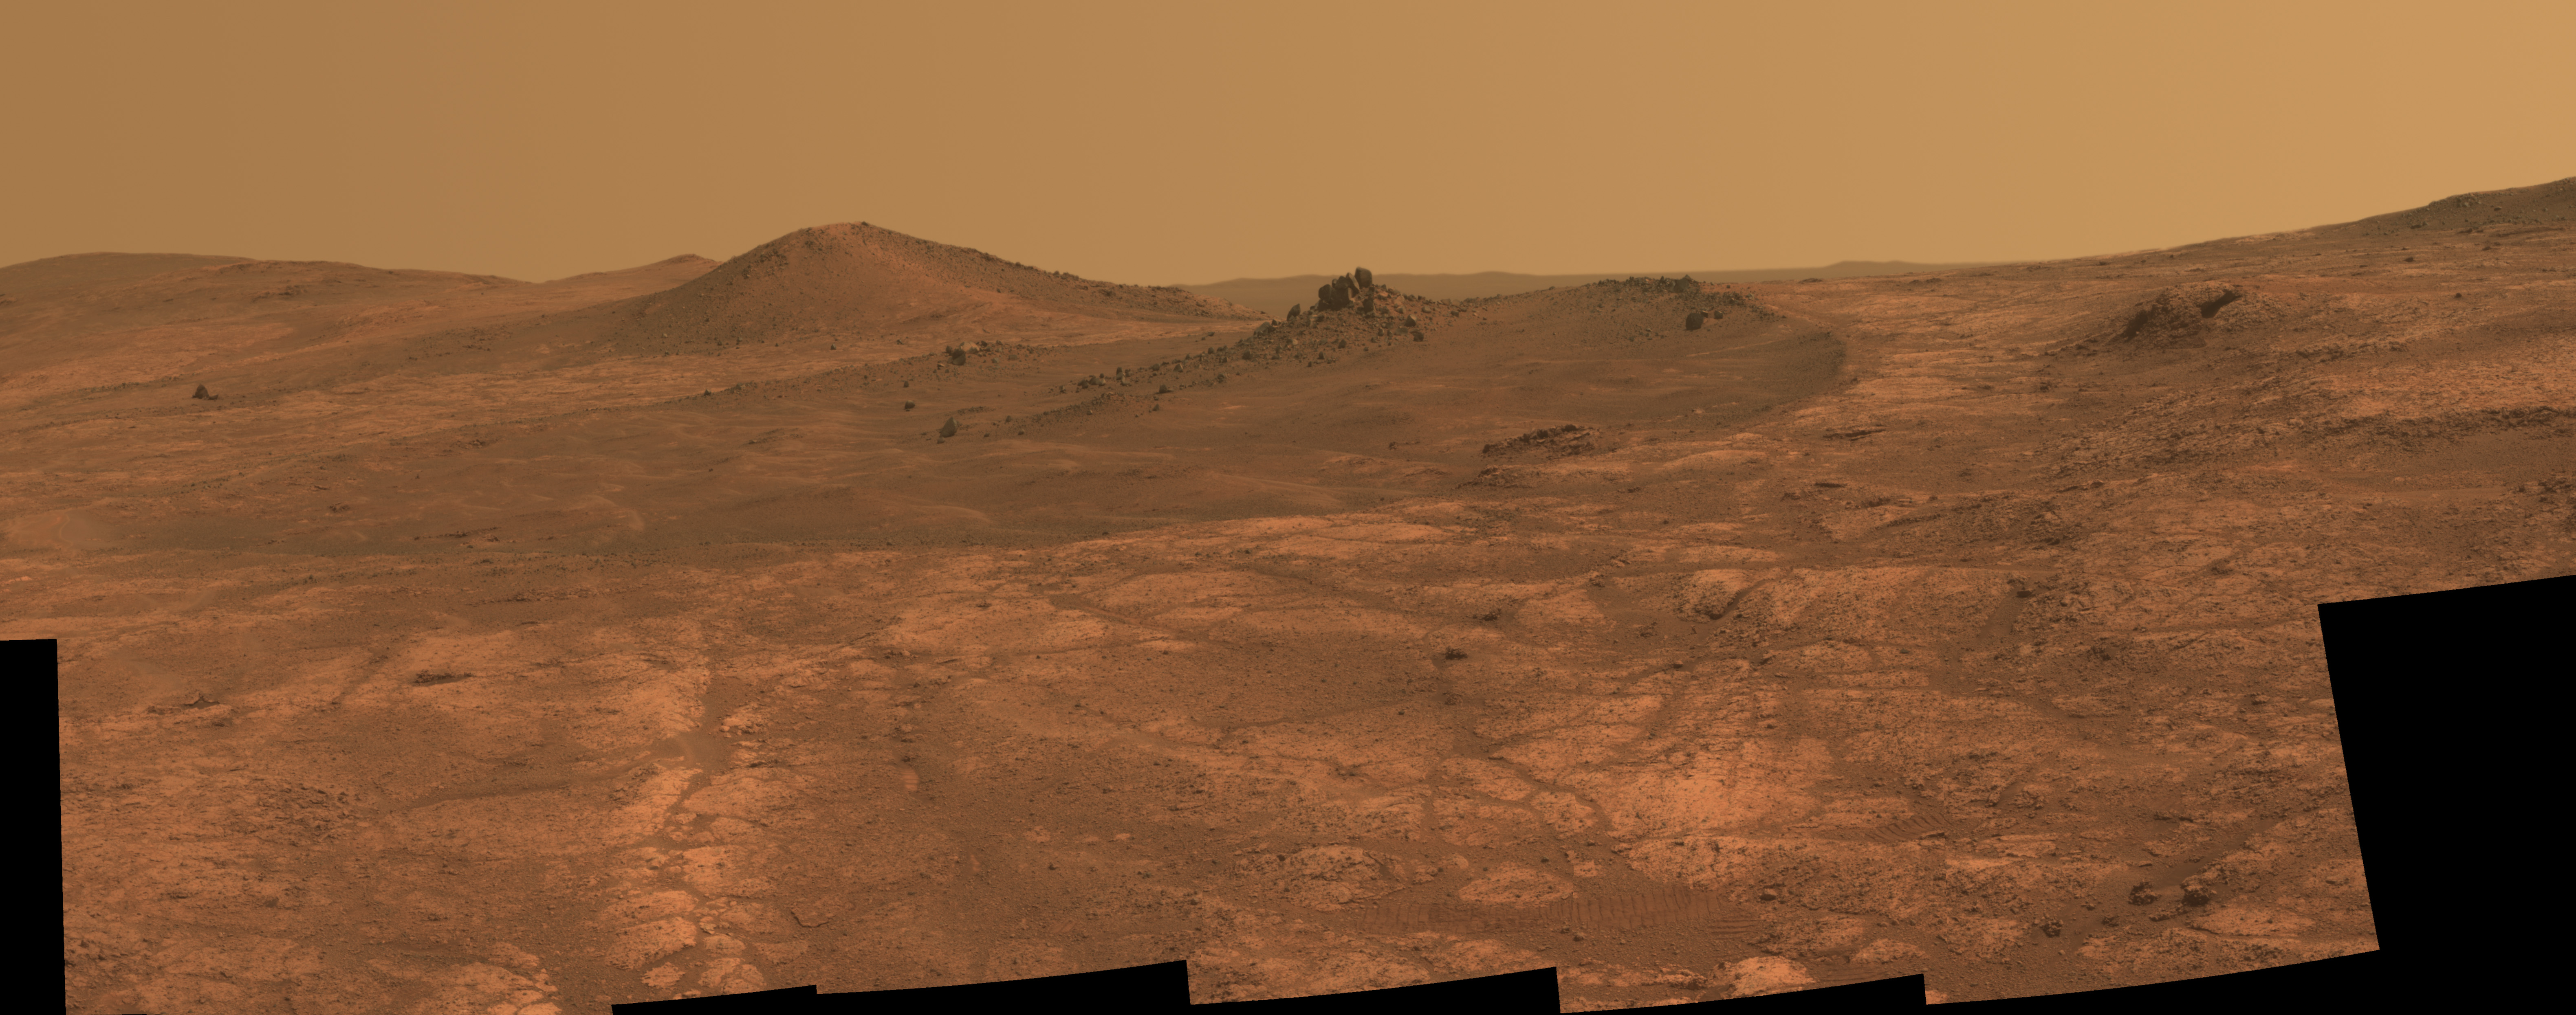
\includegraphics[width = \textwidth]{image_mars_elongated_crater}
		\caption{Elongated crater ``Spirit of St. Louis'' on Mars taken from the panoramic camera on NASA's Mars Exploration Rover Opportunity. (Image credit: \cite{Greicius:2015})}
		\label{fig:image_mars_elongated_crater}
	\end{subfigure}
	
	\hfill
	
	\begin{subfigure}[b]{0.96\textwidth}	%0.96
		\centering
		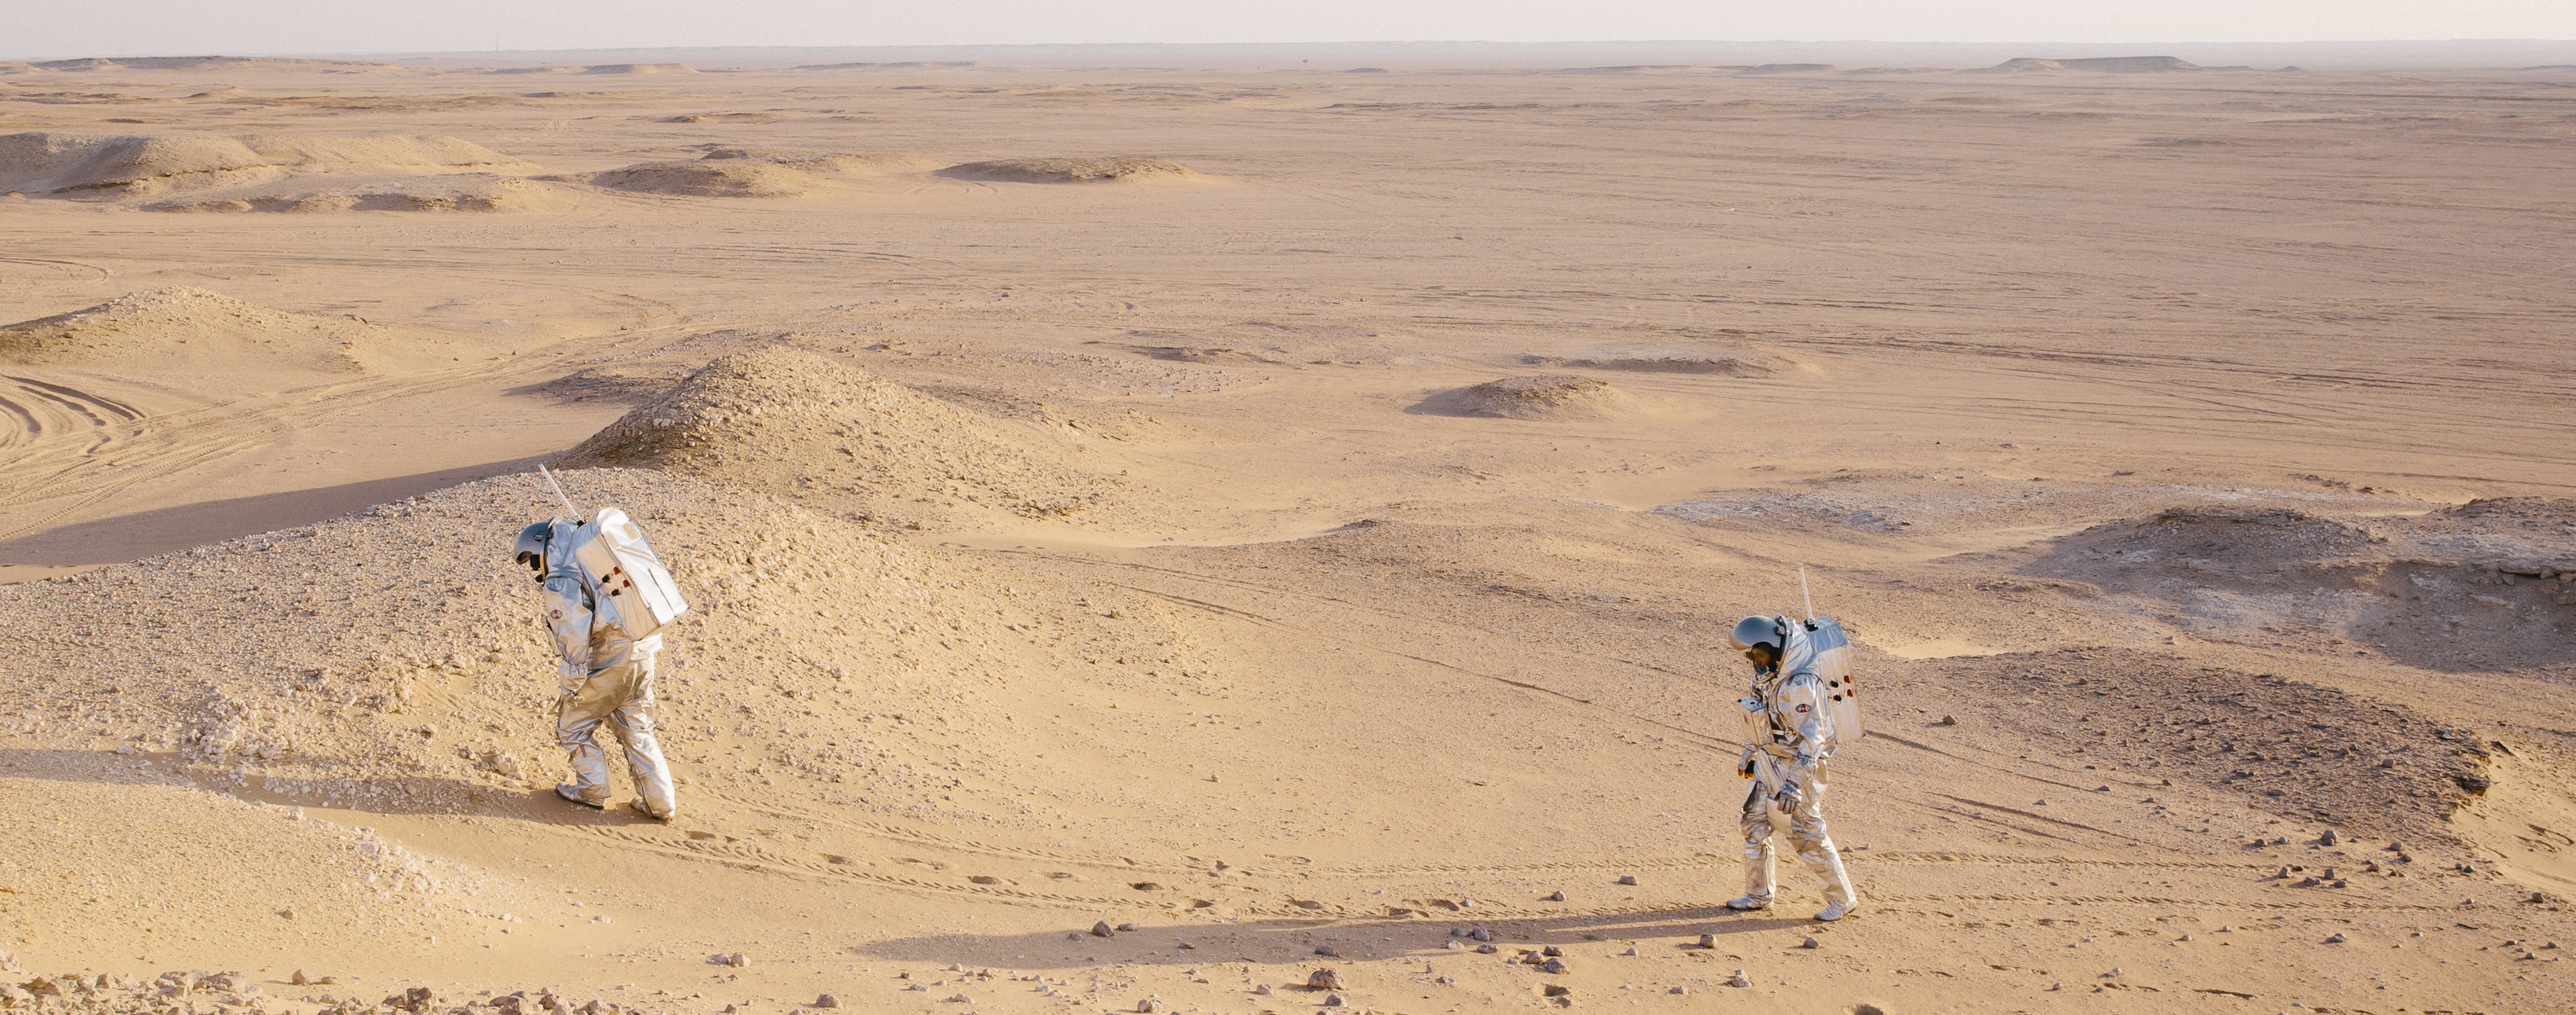
\includegraphics[width = \textwidth]{image_oewf_oman}
		\caption{Two analog astronauts from the OeWF performing a simulation with Aouda spacesuit simulators in the Dhofar Desert in Oman. (Image credit: OeWF/Florian Voggeneder)}
		\label{fig:image_oewf_oman}
	\end{subfigure}
	\caption{Visible geological similarities between the Martian surface and an analog Martian environment on Earth.}
	\label{fig:analogy_mars_oman}
\end{figure}
\vfill

With the help of Aouda, analog astronauts can conduct basic training, experiments and other important tasks while experiencing similar restrictions and technical aids a Mars spacesuit in two to three decades will have. This makes it possible to collect vital data from different scientific areas, which can help future astronauts to safely prepare for Mars missions \cite{OeWF:2019_history}.

In 2010, the Aouda spacesuit simulator was tested for the first time in a field simulation on a glacier in the Kaunertal in Austria. The mission lasted for two days and aimed to perform astrobiological experiments. Further missions took place in 2011 in Rio Tinto in Spain, in 2012 on the Dachstein mountains in Austria, in 2013 in the northern Sahara near Erfoud in Morocco (MARS2013), in 2015 again in the Kaunertal in Austria (AMADEE-15) and in 2018 in the Dhofar Desert in Oman (AMADEE-18). The next mission, called AMADEE-20, was planned to take place in late 2020 in the Negev Desert in Israel but it was postponed until October 2021 due to the ongoing SARS-CoV-2 pandemic. Missions carried out by the OeWF generally last from a couple of days to a few months \cite{OeWF:2019_missions, Israel:2020}.

\section{Serenity spacesuit simulator}
After ten years and more than 750 hours of \emph{extravehicular activities} (EVAs), Aouda's successor is the Serenity spacesuit simulator. In participation with national and international high-end universities and companies, Serenity has been under development since 2018. Bernhard Kaliauer Design Studio's first concept of Serenity is shown in figure the \ref{fig:serenity_design_study}.
\begin{figure}[h!]
	\centering
	\begin{subfigure}[b]{0.47\textwidth}
		\centering
		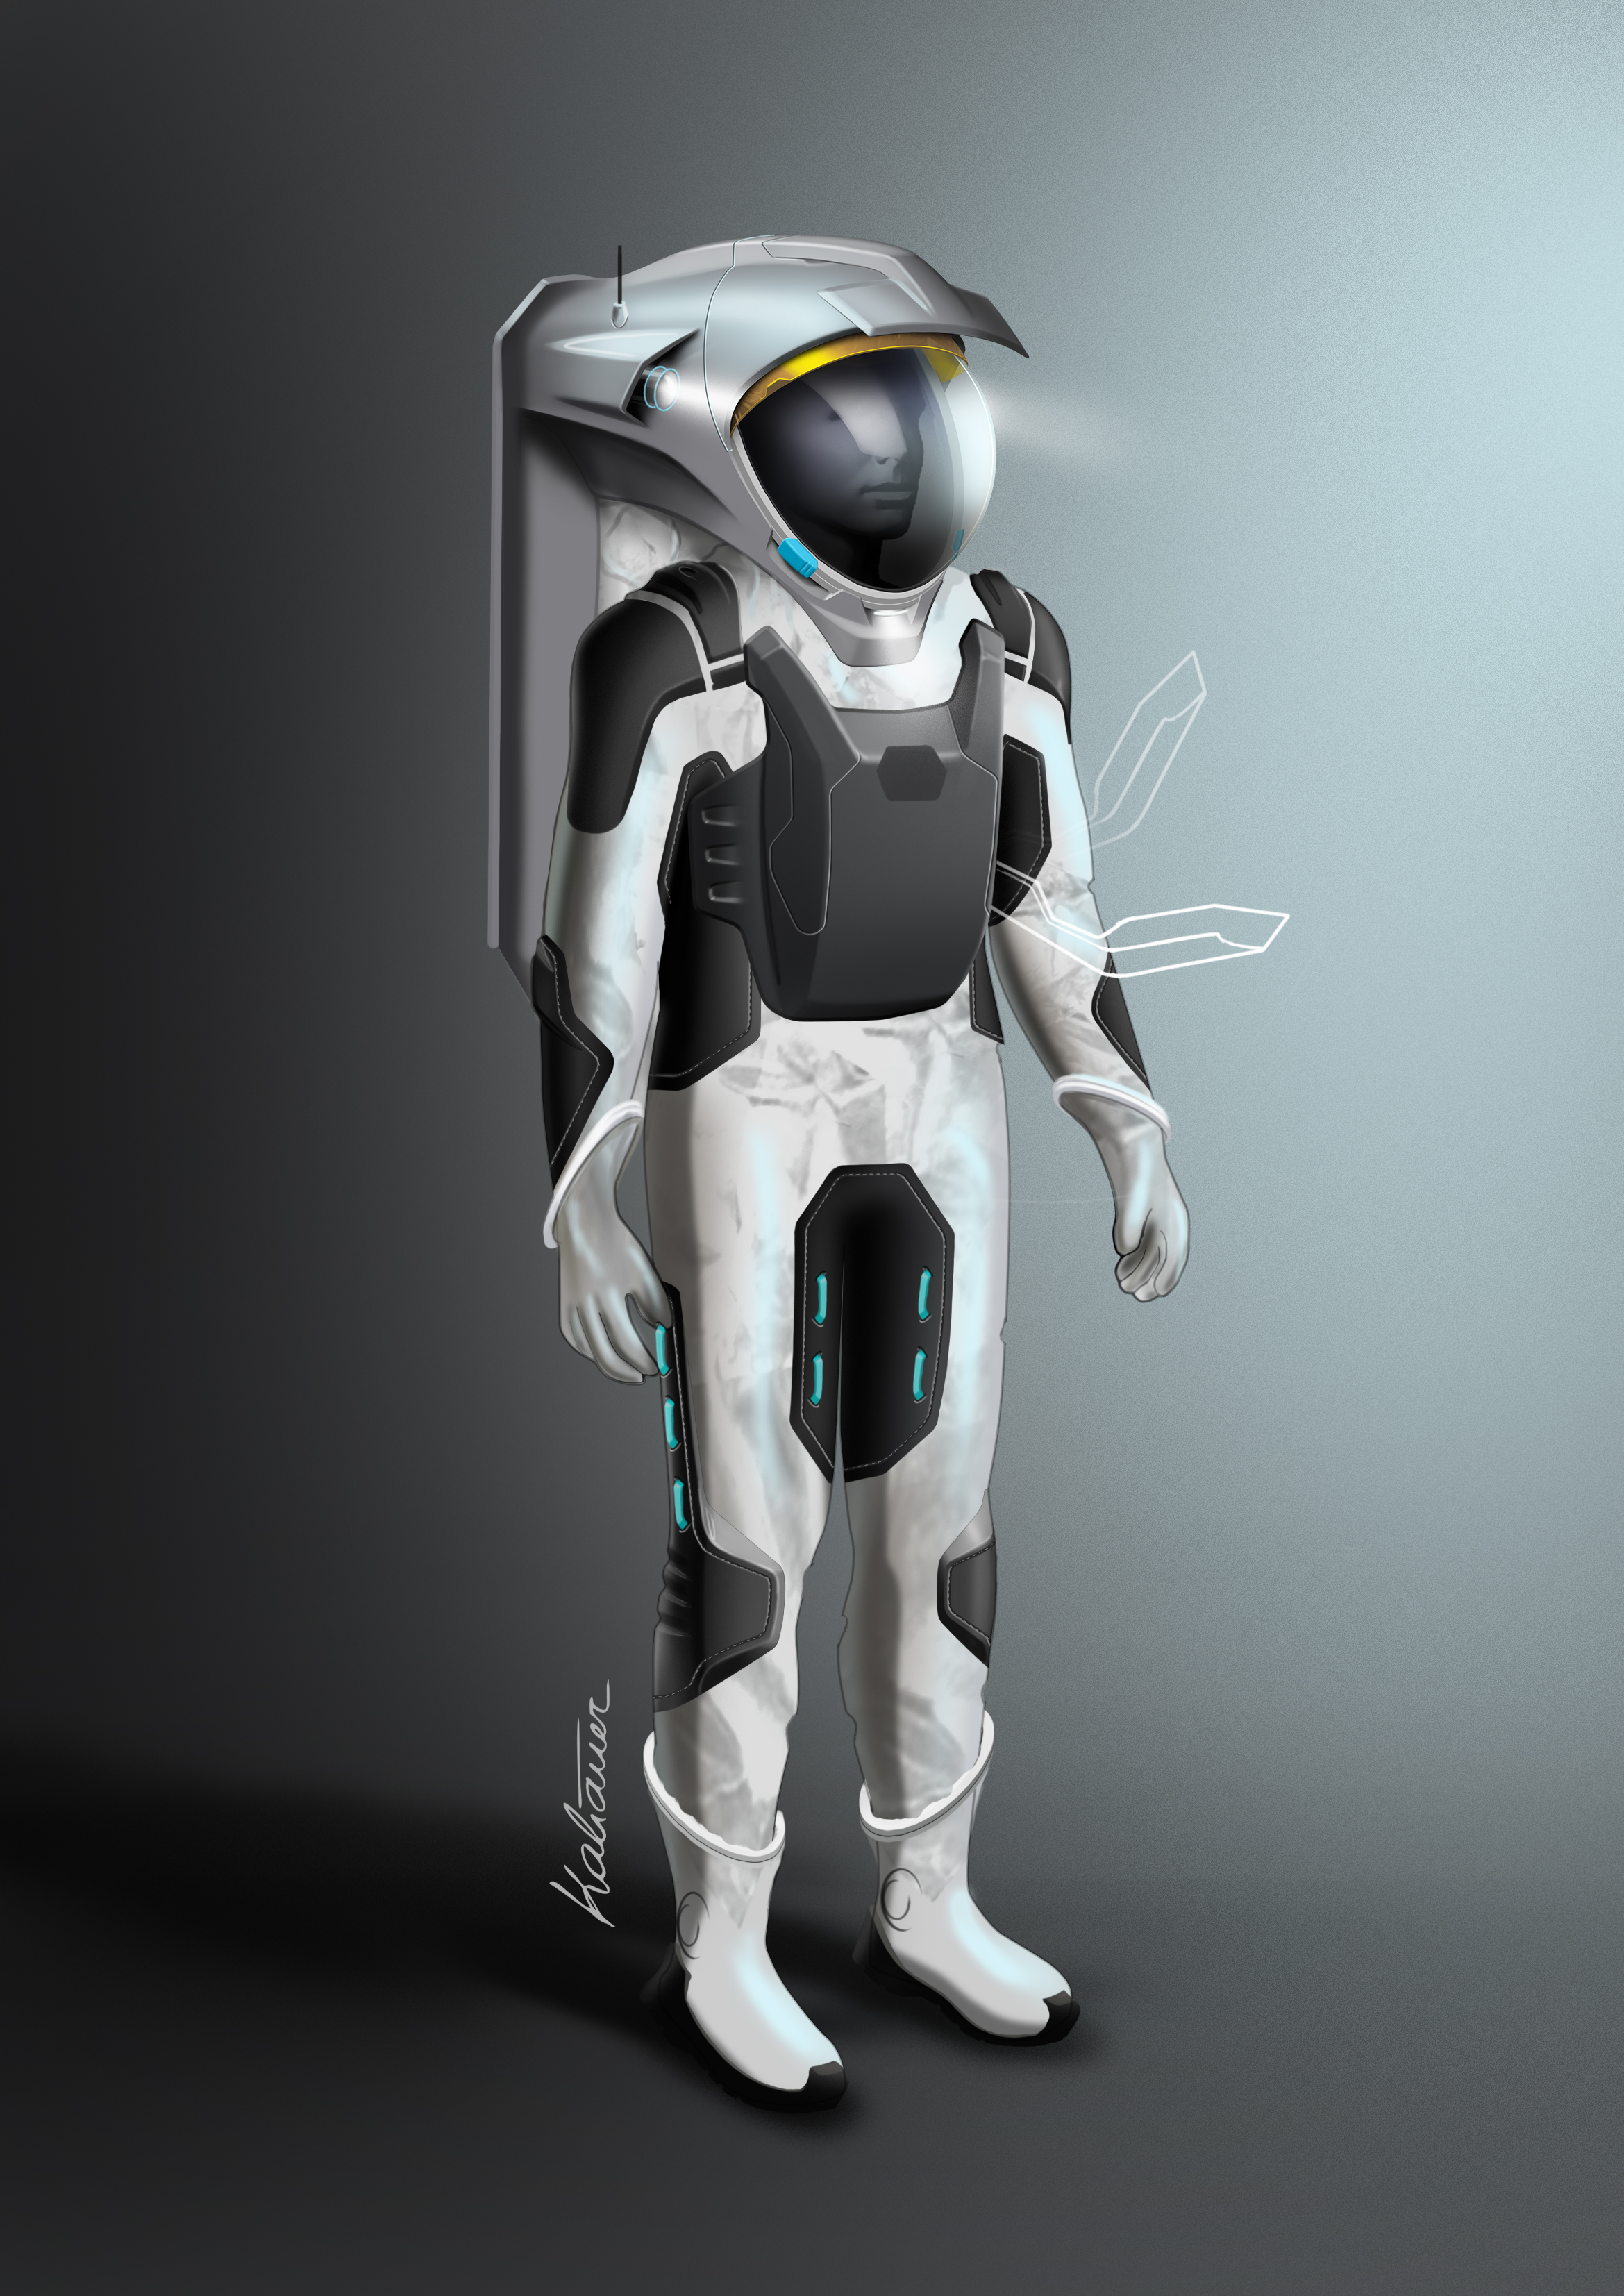
\includegraphics[width = \textwidth]{image_serenity_front_view}
		\caption{Front view}
		\label{fig:image_serenity_front_view}
	\end{subfigure}
	\hspace{5pt}%
	\begin{subfigure}[b]{0.47\textwidth}
		\centering
		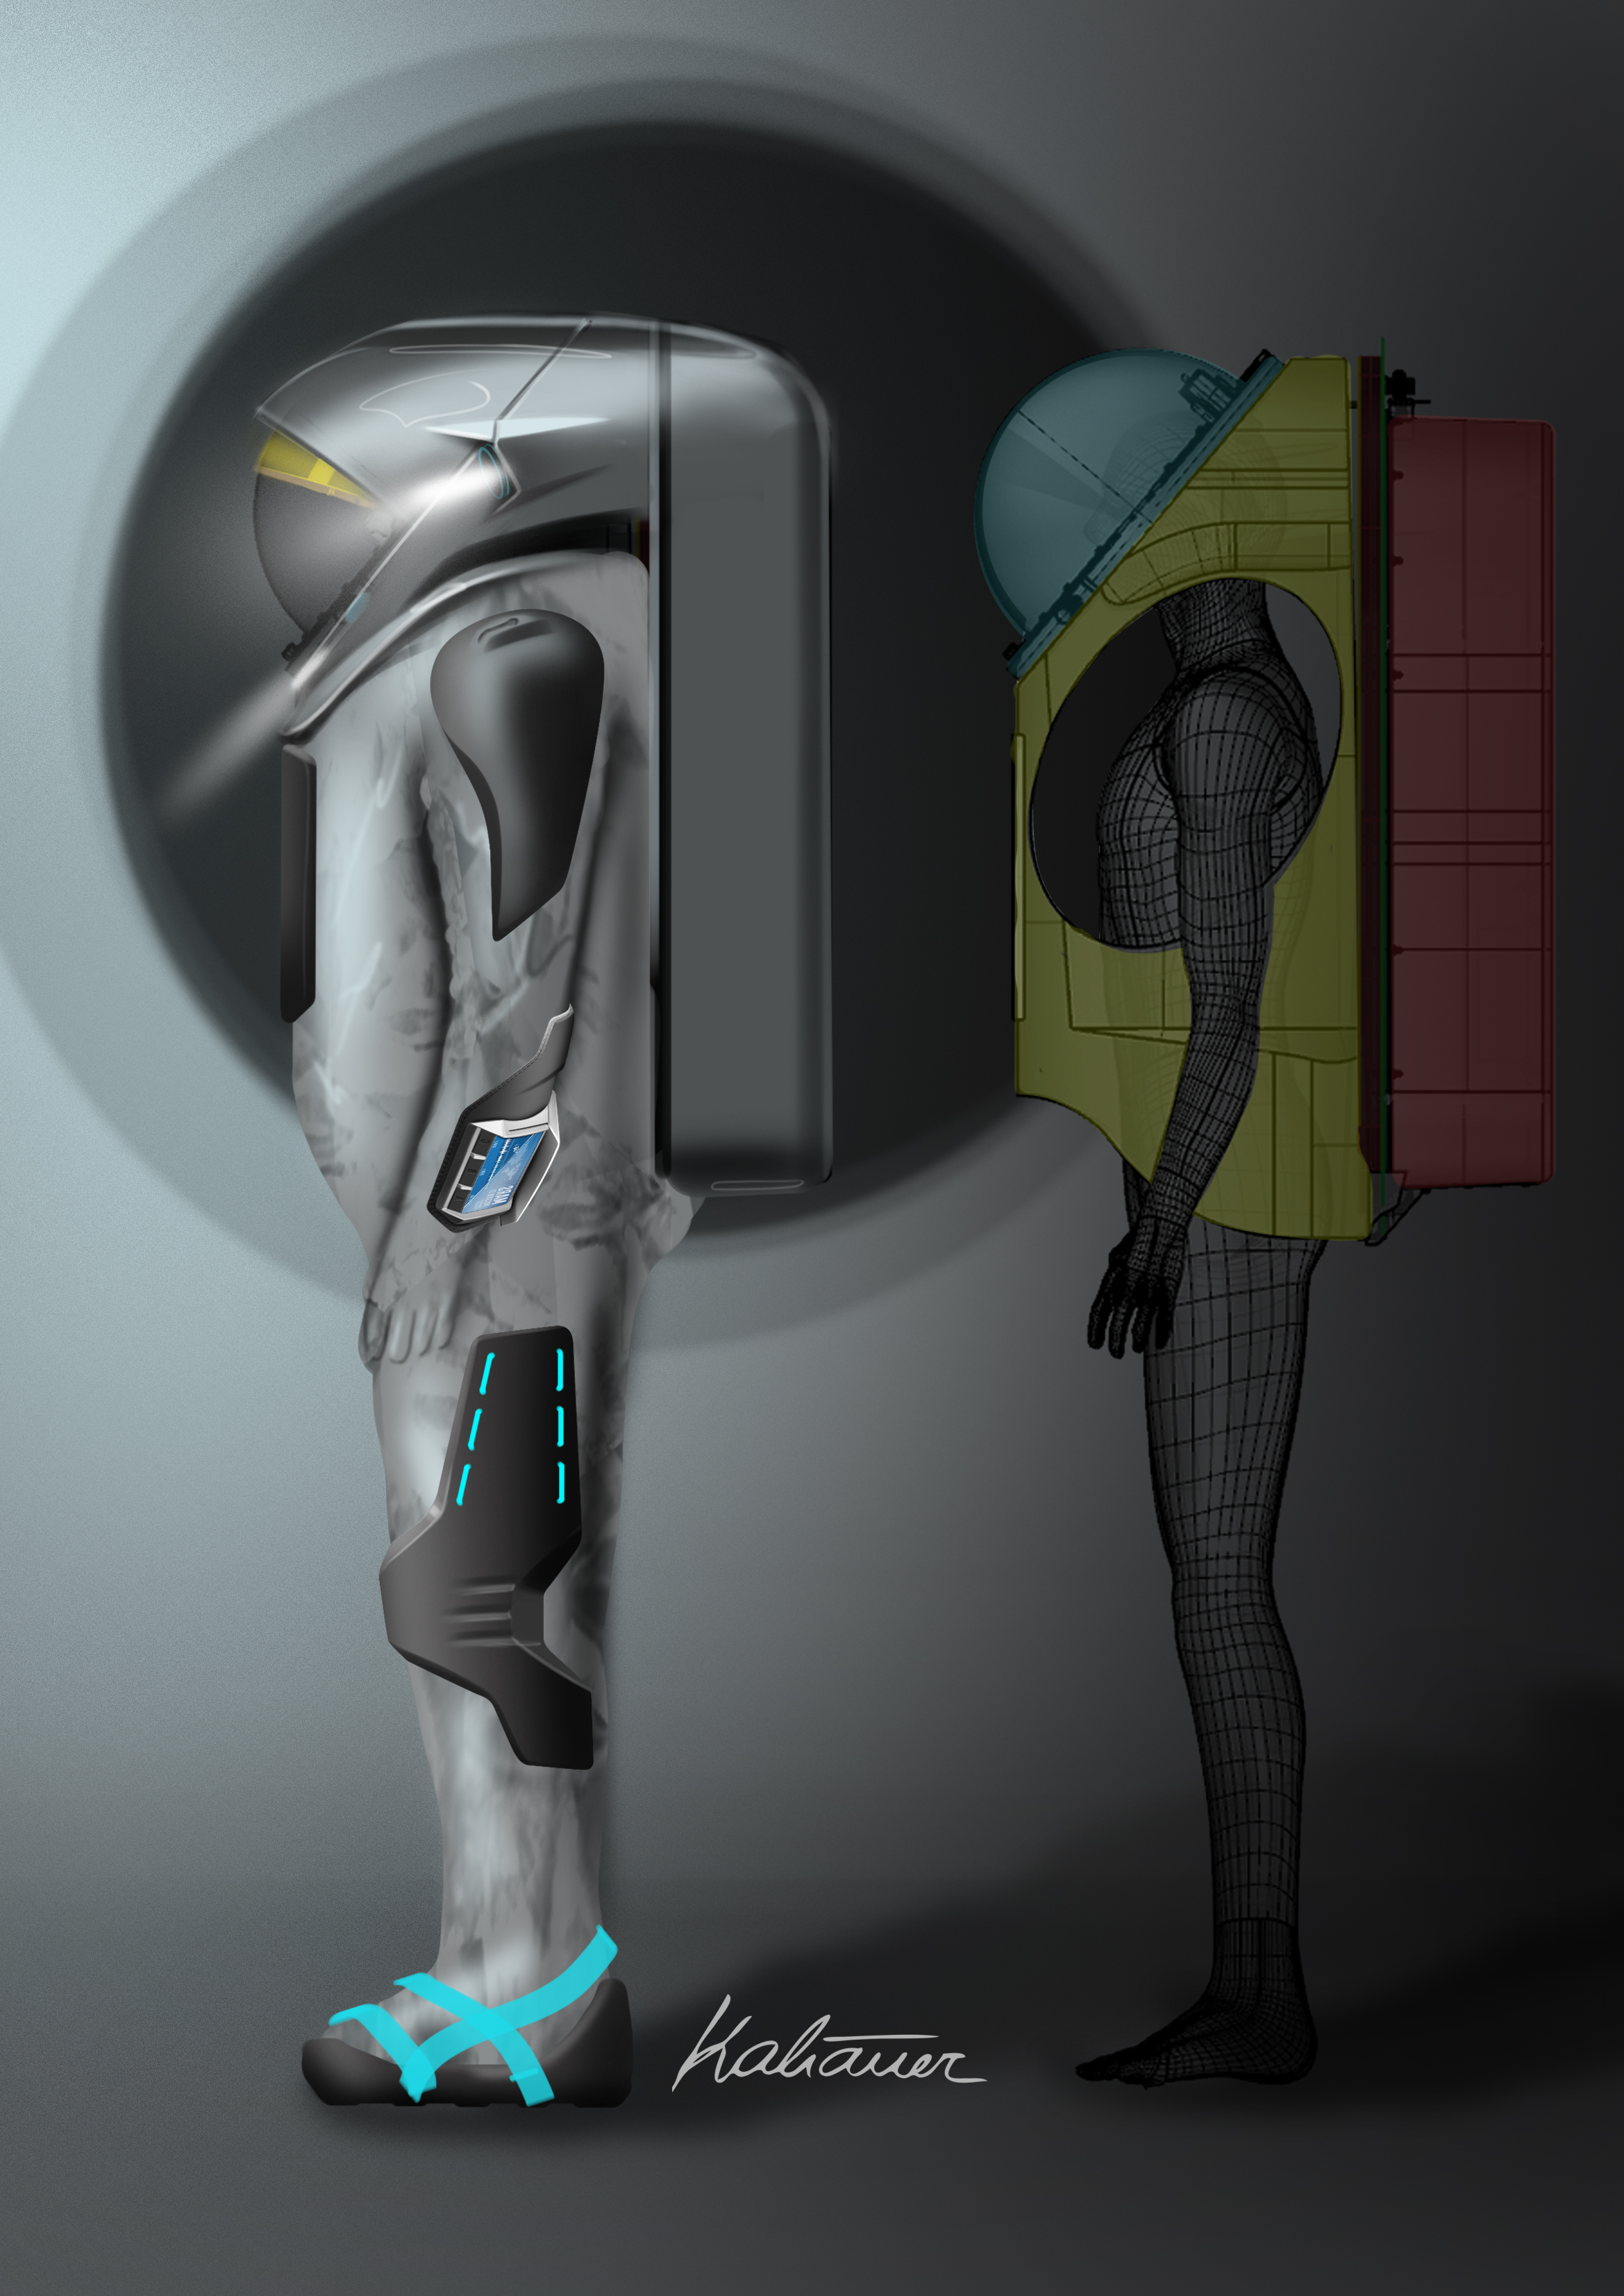
\includegraphics[width = \textwidth]{image_serenity_side_view}
		\caption{Side view}
		\label{fig:image_serenity_side_view}
	\end{subfigure}
	\caption{Serenity spacesuit simulator design study. (Image credit: OeWF/Bernhard Kaliauer Design Studio)}
	\label{fig:serenity_design_study}
\end{figure}

It is important to the OeWF to make the transition from Aouda to Serenity as fluid and environmentally friendly as possible. That is why, on the one hand, tried and tested materials are being upgraded and re-used, which shortens the retraining time of the analog astronauts, and on the other hand, a number of innovations are introduced based on the knowledge gathered over the past few years. 

Apart from the complete revision to carry out even more realistic simulations, a new advanced rear-entry system will be implemented. This system represents the latest NASA standard for Mars missions due to its ability to easily dock at a habitat, thus reducing contamination and donning time \cite{EVA:2018}.

